\chapter{Replication}
\lecture{5}{10/2}

\begin{definition}[Replication]
    \textbf{Replication} involves providing multiple copies of the same data
    or serves in a distributed system.
\end{definition}

Replication improves system capabilities in terms of performance
(for example, web caching),
availability
(having data stored in multiple places in case of server failures),
and load distribution
(avoid servers being overloaded).

We have two types of replication:
\begin{enumerate}
    \item \textbf{computation replication}: having multiple
        instances of the same functional process being executed; and
    \item \textbf{data replication}: the same piece of information is
        being stored on multiple devices.
\end{enumerate}

When implementing replication, we must meet the following requirements:
\begin{enumerate}
    \item \textbf{replication transparency}: a user can see the logical service
        provided to it, but not the multiple physical copies of the
        service running; and
    \item \textbf{data consistency}: the same request should receive the same
        result even if it is being processed by a different copy of the same
        service.
\end{enumerate}

\begin{definition}[Replicas]
    We call copies of the same data or functions \textbf{replicas}.
\end{definition}

Replicas may not \emph{always} be consistent,
some may have received updates that has not yet been conveyed to the others.
These replicas may be implemented by different technologies, 
as long as we have replication transparency and data consistency.

Within a distributed system, we can look at three different types of components:
\begin{enumerate}
    \item replicas (we have already seen);
    \item clients; and
    \item the front end.
\end{enumerate}
Our workflow may look as follows:
\begin{enumerate}
    \item the front end receives a request from a client,
        this request is forwarded to the replicas;
    \item the replicas will accept the request
        and will decide the ordering of the request relative to other requests;
    \item once the request's time to execute has come,
        the replicas will process the request;
    \item the replicas will reach a consensus on the effect of the requests; and
    \item finally one or more of the replicas will respond to the front end,
        the front end may process the response before returning it to the client(s).
\end{enumerate}

\begin{definition}[Fault-tolerant service]
    A \textbf{fault-tolerant service} is a service that will continuing providing
    \emph{correctly} despite up to $f$ process failures.
\end{definition}

Replicas in a system are assumed to behave according to the \emph{specification}
if the distributed system.

\begin{example}
    A specification of bank accounts should ensure that funds
    transferred between bank accounts can \emph{never} disappear.
    Furthermore, only deposits and withdrawals can affect the balance
    of an account.
\end{example}

A service is said to be \textbf{correct} if:
\begin{enumerate}
    \item it keeps respondining despite failures; and
    \item if clients cannot tell the difference between the service
        they obtain from an implementation with repllicated data 
        and one provided by a single correct replica manager.
\end{enumerate}

\begin{definition}[Primary-backup model]
    The \textbf{primary-backup model}
    (or \textbf{passive model}) is a distributed systems model for fault tolerance
    where, at any given time, there is a single primary replica
    and one or more secondary (backup) replicas.
    The front end will communicate with the primary replica,
    which will execute the operations and send the copies of the updated data
    to the backups.
    If the primary replica fails, one of the backups is promoted to act as the primary.
\end{definition}

\begin{figure}[]
    \centering
    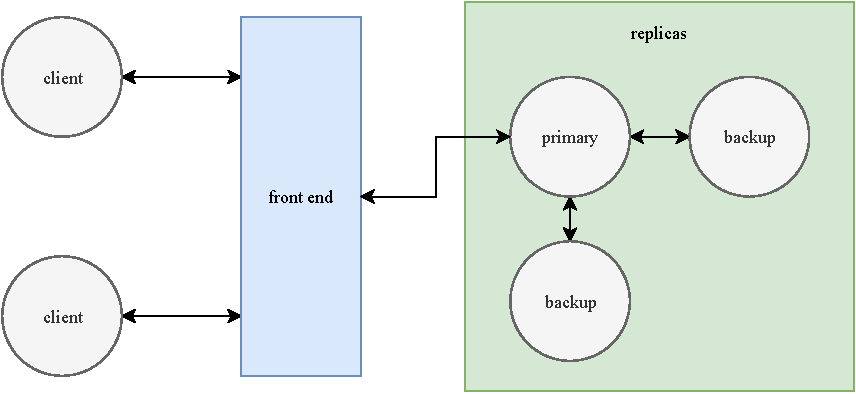
\includegraphics[width=0.8\linewidth]{images/primary-backup.pdf}
    \caption{A diagram showing how the primary-backup model works.}%
    \label{fig:primary-backup}
\end{figure}

Let's look at the workflow for passive replication:
\begin{enumerate}
    \item the front end issues the request, containing a unique identify,
        to the primary replica;
    \item the primary replica will process each request \emph{in the order} in which
        it receives, it will check the unique id and if it has already done
        the request it will resend the response;
    \item the primary replica, if not done already, will execute the request and
        store the response;
    \item if the request is an update, the primary replica will send
        the updated data to the backup replicas
        (the backup replicas will send an acknowledgement); and
    \item the primary replica will respond to the front end, which will
        in turn hand the respond (with some possible transformation)
        back to the client.
\end{enumerate}

A distributed system implementing passive replication with $f$ replicas
can survive up to $f - 1$ replica crashes.
Passive replication requires little functionality, 
you only need to lookup a new primary replica when the current has crashed;
however, there is a large system overhead due to data propagation.

\begin{definition}[Active replication]
    In \textbf{active replication}, each request is processed by every replica
    at the same time.
\end{definition}

\begin{figure}[]
    \centering
    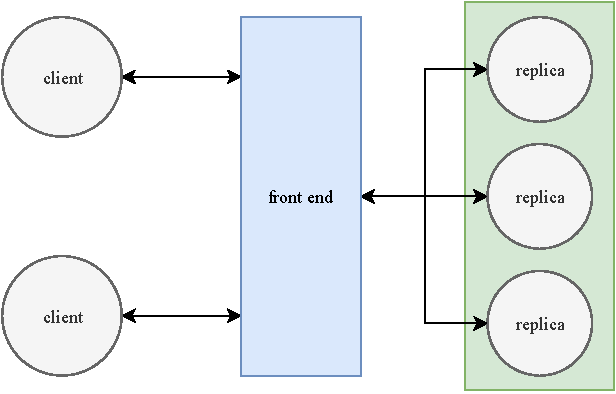
\includegraphics[width=0.8\linewidth]{images/active-replication.pdf}
    \caption{A diagram illustarting active replication in a distributed system.}%
    \label{fig:active-replication}
\end{figure}

Let's look at the workflow for active replication:
\begin{enumerate}
    \item the front end will attach a unique identifier to a request
        and the cast them to all of the replicas;
    \item the replicas will receive the request in the same order;
    \item every replica will execute the request, and places the identifier in
        the response;
    \item there is \emph{no} agreement;
    \item the front end will collect responses frmo the replicas and may use
        one or more of the responses
        (if it is only trying to tolerate crash failures it gives the client
        the first response).
\end{enumerate}
The front end uses a \emph{totally ordered reliable multicast} to send
requests to the replicas to ensure that the requests are received in the
same total order.

\begin{definition}[Byzantine fault]
    A \textbf{Byzantine fault} is an arbitrary fault that occurs during
    the execution of an algorithm in a distributed system.
    It includes:
    \begin{enumerate}
        \item \textbf{omission failures}: for example
            crash failures, failing to receive a request, or failing to send a
            response; and
        \item \textbf{commission failures}: for example
            processing a request incorrectly, corrupted local state,
            sending an incorrect or inconsistent response to a request.
    \end{enumerate}
\end{definition}

We characterise \emph{Byzantine failure-tolerant algorithms} by
their \textbf{resilience} $f$,
this is the number of faulty processes with which the algorithm can cope.

In order to implement active replication, 
we must have a solution to a totally ordered and reliable multicast.
A system of $f$ replicas can mask up to 
$\left\lfloor \frac{f - 1}{2} \right\rfloor$.
The front end waits until it has collected $f + 1$ \emph{identical}
responses and passes that response back to the client, discarding
the other responses.
The front end may only send read-only request to individual replica.
This loses fault tolerance, but remains sequentially consistent.
We can easily mask replica failure in this case,
by submitting the read-only request to another replica.
